\documentclass[sigconf,review,anonymous]{acmart}

\setcopyright{none}
\settopmatter{printacmref=true}
\renewcommand\footnotetextcopyrightpermission[1]{}

\acmConference[ETRA '27]{ACM Symposium on Eye Tracking Research \& Applications}{2027}{Pamplona, Spain}
\acmYear{2027}

\usepackage{booktabs}
\usepackage{graphicx}
\usepackage{microtype}
\usepackage{tikz}
\usepackage{xcolor}
\usetikzlibrary{arrows.meta,fit,positioning}

\definecolor{draftred}{RGB}{150,30,30}
\newcommand{\draftnote}[1]{\textcolor{draftred}{\textbf{[Draft note: #1]}}}

\graphicspath{{../Master-Thesis-Report/}}

\title{Reading the Reader: An Auditable, Modular Platform for Real-Time Gaze-Contingent Reading Experiments}

% The working draft is anonymous because ETRA uses double-blind review.
% Confirm the complete author list and order with the supervisory team before submission.
\author{Anonymous Author(s)}

\begin{abstract}
Gaze-contingent reading studies often rely on tightly coupled prototypes in which sensing, eye-movement analysis, adaptation logic, and presentation are difficult to replace or inspect independently.
This limits systematic comparison of interventions and makes it hard to reconstruct why a change was shown to a reader.
We present \emph{Reading the Reader}, a researcher-operated platform that separates sensing, analysis, decision, and intervention behind versioned in-process and out-of-process contracts.
A participant reads on one display while a researcher monitors gaze and controls manual, advisory, or autonomous interventions on another.
The system can defer validated typographic changes to sentence, paragraph, or page boundaries, capture a semantic reading anchor across layout reflow, and record raw gaze, derived events, proposals, interventions, and performance telemetry on one replayable timeline.
We evaluate the artifact through architecture tests and external-provider integrations, eight Tobii-backed reading sessions, and a deterministic restoration benchmark.
Across the eight sessions, gaze acquisition averaged 89.9 Hz with 95.6\% mean validity; local participant and researcher transport had 95th-percentile round trips of 3 and 8.4 ms.
A separate 91-second advisory run measured a 95th-percentile decision-path time of 11 ms and provider round trips no greater than 7 ms.
Instrumentation also exposed systematic over-positioning in the original restoration strategy and motivated an offset-preserving revision.
The results support the platform as an auditable instrument for developing gaze-contingent reading experiments; the small exploratory participant sample is not used to claim reading efficacy.
\end{abstract}

\ccsdesc[500]{Human-centered computing~Human computer interaction (HCI)}
\ccsdesc[300]{Human-centered computing~Empirical studies in HCI}
\ccsdesc[300]{Software and its engineering~Software architectures}

\keywords{eye tracking, adaptive reading, gaze-contingent interaction, research platform, auditability, typographic intervention}

\begin{document}
\maketitle

\section{Introduction}

Digital text can change while it is being read.
Font size, line width, spacing, contrast, and typeface can be adjusted to a reader's needs, and eye tracking provides a signal from which a system can estimate where the reader is looking and when an adaptation may be appropriate.
This creates the possibility of a closed-loop reading interface: sense gaze, interpret reading behavior, decide whether to intervene, and alter the presentation in real time.
The premise is especially relevant to accessible reading, where adjustable typography can support low-vision readers and where layout parameters affect online readability \cite{arditi2004adjustable,beier2021letterspacing,rello2016makeitbig}.

Building a single adaptive reader, however, is different from building an instrument with which adaptive reading can be studied.
A scientific platform must permit a researcher to exchange a tracker or event detector, compare decision strategies, control when an intervention is committed, and recover the evidence that explains every visible change.
Earlier work in the Reading the Reader program demonstrated gaze collection, typographic intervention, and reactive interfaces, but did so through largely self-contained prototypes that evolved by extending earlier applications \cite{refsgaard2024rtr,pereira2024typography,palinec2024reactive}.
That organization makes a new intervention possible, but makes interventions and decision strategies difficult to compare without changing the runtime that presents and measures them.

The human-computer interaction problem is equally important.
A change in font size or line width can reflow the document and displace the word or sentence being read.
Prior work within the program showed that intervention form and highlighting affect reading recovery and preference \cite{jensen2025context}.
More broadly, gaze-contingent highlighting can change reading behavior \cite{rummens2025highlighting}, while gaze-driven interfaces such as eyeBook and New Line illustrate alternative ways of using gaze during reading \cite{biedert2010eyebook,medan2024newline}.
An experiment platform therefore should not treat presentation as a stateless actuator.
It must know \emph{when} a change is safe to commit, preserve or at least measure the reader's place across the change, and keep the researcher in control of uncertain decisions.

We present \emph{Reading the Reader}, a dual-screen platform for real-time gaze-contingent reading experiments.
The platform decomposes the adaptive loop into four modules--sensing, eye-movement analysis, decision, and intervention--behind stable application ports and a versioned WebSocket provider protocol.
The participant surface maps gaze to the rendered document and applies bounded typographic changes.
The researcher surface mirrors the reader, visualizes gaze and derived events, and supports manual intervention or approval of external proposals.
A backend session authority records raw and enriched samples, proposals, approvals, applied interventions, context-restoration outcomes, and telemetry on a common timeline.

This paper makes three contributions:

\begin{enumerate}
    \item \textbf{A modular experiment architecture} that separates the four stages of gaze-contingent adaptation while supporting built-in and out-of-process implementations and a two-screen researcher-in-the-loop workflow.
    \item \textbf{A boundary-aware intervention and evidence mechanism} that validates typographic changes, stages layout-affecting actions at reading boundaries, captures semantic anchors across reflow, and records both the action and its measured restoration outcome.
    \item \textbf{An artifact evaluation} combining executable architecture evidence, provider integrations, real-hardware sensing and latency measurements, and a failure-driven case study in which the instrumentation exposed over-positioning in the original restore strategy.
\end{enumerate}

The evaluation is deliberately an evaluation of the research instrument.
Four participants completed two feasibility sessions each, but interventions were manually timed and the enabled condition bundled position restoration with highlighting.
We report those behavioral observations descriptively and make no claim that the platform or an intervention improves reading speed, comprehension, or accessibility.

\section{Related Work}

\subsection{Eye Movements and Interactive Reading}

Eye movements provide a temporally rich account of reading.
Fixations are periods in which useful visual information is acquired, saccades move the eyes between locations, and regressions move against the normal reading direction.
Foundational accounts relate fixation behavior to ongoing language processing \cite{just1980reading}, and reviews synthesize how fixation duration, saccade patterns, and regressions reflect reading and attention \cite{rayner1998eyemovements,rayner2009eyemovements}.
Operational systems must first reduce raw gaze to events, and event-identification approaches differ in whether they use velocity, dispersion, or areas of interest \cite{salvucci2000identifying}.

Interactive reading systems move gaze analysis from post-hoc measurement into the interface loop.
The eyeBook used gaze position to provide contextual feedback during reading \cite{biedert2010eyebook}.
New Line presented text in a continuous gaze-controlled line and emphasized the current word \cite{medan2024newline}.
Rummens and Beier dynamically colored the fixated word for beginning readers and found changes in reading efficiency without a corresponding preference for the dynamic presentation \cite{rummens2025highlighting}.
These systems demonstrate the design space for gaze-driven support, but they primarily instantiate and evaluate a particular interaction.
Our focus is the reusable experimental boundary around sensing, analysis, decisions, and interventions.

Accurate online mapping from gaze to multiline text remains difficult because tracker noise, calibration drift, regressions, and ambiguous line geometry affect assignment.
Recent confidence-based line assignment explicitly models uncertainty and can defer low-confidence assignments \cite{kaltenberger2026confla}.
The present platform instead implements a lightweight browser-side geometric heuristic with smoothing, dwell, and token hysteresis.
We treat this as a replaceable analysis component rather than a new fixation or line-assignment algorithm.

\subsection{Adaptive Typography and Context Preservation}

Typography influences the reading task.
Studies have examined font size and line spacing \cite{rello2016makeitbig}, typeface and size under eye tracking \cite{beymer2008eyetracking}, letter spacing and width for low-vision readers \cite{beier2021letterspacing}, and adjustable typography as an accessibility mechanism \cite{arditi2004adjustable}.
The Reading the Reader program translated these parameters into interactive interventions.
Earlier prototypes collected gaze, applied typographic adjustments, and explored popup, undo, notification, and gradual forms \cite{refsgaard2024rtr,pereira2024typography,palinec2024reactive}.

Jensen et al. subsequently foregrounded the recovery problem: an adaptive change may help in the long term while interrupting the reader at the moment it is applied.
Their ETRA study introduced explicit context highlighting and the reading-resume-time metric, and compared intervention designs in a 22-participant study \cite{jensen2025context}.
This paper addresses the systems question that follows from that empirical work: how can an experiment runtime schedule a layout-changing intervention, preserve a semantic position across reflow, and produce enough evidence to determine when preservation itself fails?

\subsection{Experiment Platforms and Auditable Adaptation}

PsychoPy and Psychtoolbox are established tools for behavioral experiment construction and stimulus delivery \cite{peirce2019psychopy,brainard1997psychtoolbox}.
They support broad experiment designs and hardware integration, but a gaze-contingent adaptive reader still requires study-specific logic for semantic text mapping, proposal handling, controlled reflow, and recovery measurement.
Commercial eye-tracking suites similarly emphasize experiment design, recording, and post-hoc analysis rather than a replaceable live decision layer.

Our architecture applies ports-and-adapters and dependency inversion \cite{cockburn2005hexagonal,martin1996dip,martin2017cleanarch} to make that live decision boundary explicit.
The contribution is not the architectural pattern by itself.
It is its realization as an experiment instrument in which high-frequency gaze transport, researcher control, external module integration, layout commits, and a replayable record meet at one authoritative session boundary.

\section{Design Goals and Architecture}

The design was guided by four goals derived from the limitations of earlier prototypes and from the needs of a researcher operating a live reading study.

\begin{enumerate}
    \item \textbf{Replaceable adaptive stages.} Sensing, analysis, decision, and intervention should be independently implementable and testable. A new provider should not require changes to the central session runtime.
    \item \textbf{Inspectable real-time operation.} The gaze path should sustain the tracker's sampling rate, expose quality and latency measurements, and avoid hiding decision work inside the rendering loop.
    \item \textbf{Controlled and measurable intervention.} A layout-changing intervention should be validated, committed at an explicit reading boundary, and accompanied by a measurement of what happened to the reader's semantic position.
    \item \textbf{Researcher authority and provenance.} A researcher should be able to observe and override the system. Exported evidence should connect input, proposal, action, and outcome on a common timeline.
\end{enumerate}

\begin{figure*}[t]
    \centering
    \resizebox{\textwidth}{!}{%
    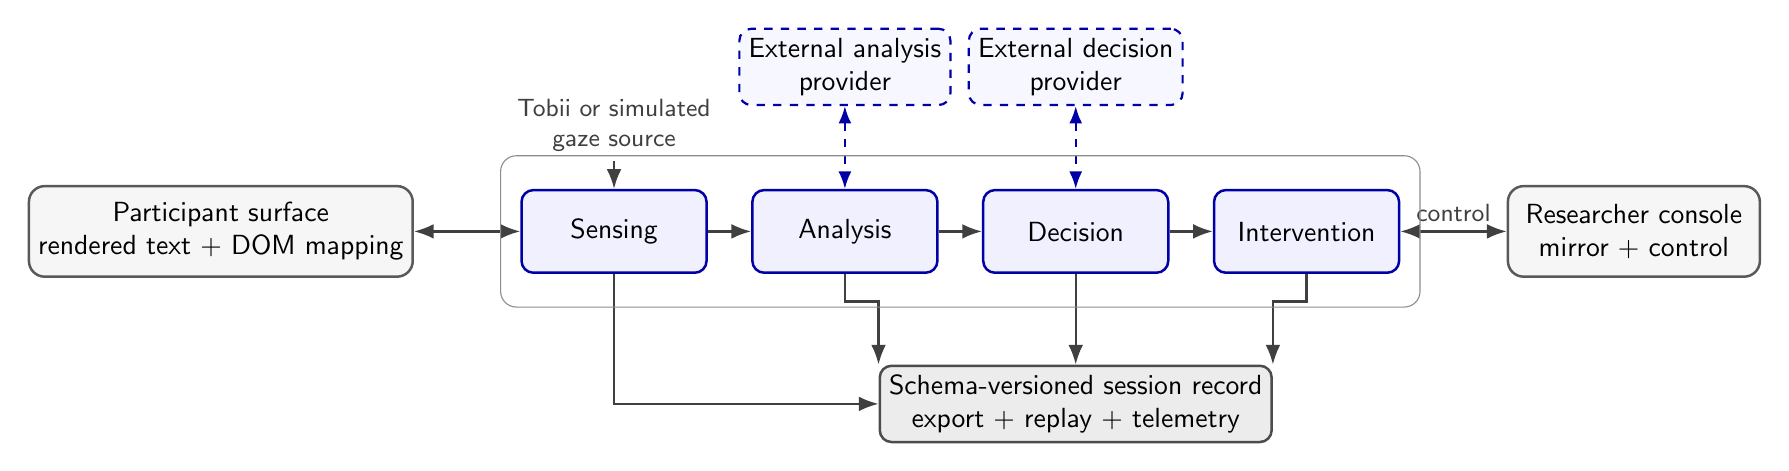
\begin{tikzpicture}[
        font=\sffamily,
        flow/.style={-{Latex[length=2.5mm]}, line width=0.8pt, draw=black!75},
        bidir/.style={{Latex[length=2.5mm]}-{Latex[length=2.5mm]}, line width=0.8pt, draw=black!75},
        providerflow/.style={{Latex[length=2.2mm]}-{Latex[length=2.2mm]}, dashed, line width=0.8pt, draw=blue!65!black},
        surface/.style={rounded corners=2mm, draw=black!65, fill=gray!7, line width=0.9pt, minimum width=3.2cm, minimum height=1.15cm, align=center},
        module/.style={rounded corners=1.5mm, draw=blue!65!black, fill=blue!6, line width=0.9pt, minimum width=2.35cm, minimum height=1.05cm, align=center},
        provider/.style={rounded corners=1.5mm, draw=blue!65!black, dashed, fill=blue!3, line width=0.8pt, minimum width=2.35cm, minimum height=0.9cm, align=center},
        record/.style={rounded corners=1.5mm, draw=black!70, fill=gray!15, line width=0.9pt, minimum width=3.1cm, minimum height=0.9cm, align=center},
        label/.style={font=\small\sffamily, text=black!75, align=center}
    ]
        \node[surface] (participant) {Participant surface\\rendered text + DOM mapping};
        \node[module, right=1.35cm of participant] (sensing) {Sensing};
        \node[module, right=0.55cm of sensing] (analysis) {Analysis};
        \node[module, right=0.55cm of analysis] (decision) {Decision};
        \node[module, right=0.55cm of decision] (intervention) {Intervention};
        \node[surface, right=1.35cm of intervention] (researcher) {Researcher console\\mirror + control};

        \node[provider, above=1.05cm of analysis] (analysisprovider) {External analysis\\provider};
        \node[provider, above=1.05cm of decision] (decisionprovider) {External decision\\provider};
        \node[record, below=1.15cm of decision] (record) {Schema-versioned session record\\export + replay + telemetry};
        \node[label, above=0.35cm of sensing] (tracker) {Tobii or simulated\\gaze source};

        \draw[flow] (tracker) -- (sensing);
        \draw[flow] (sensing) -- (analysis);
        \draw[flow] (analysis) -- (decision);
        \draw[flow] (decision) -- (intervention);
        \draw[bidir] (participant) -- (sensing);
        \draw[bidir] (intervention) -- node[above,label] {control} (researcher);
        \draw[providerflow] (analysisprovider) -- (analysis);
        \draw[providerflow] (decisionprovider) -- (decision);
        \draw[flow] (sensing.south) |- (record.west);
        \draw[flow] (analysis.south) -- ++(0,-0.35) -| (record.north west);
        \draw[flow] (decision.south) -- (record.north);
        \draw[flow] (intervention.south) -- ++(0,-0.35) -| (record.north east);

        \node[draw=black!45, rounded corners=2mm, fit=(sensing)(analysis)(decision)(intervention), inner xsep=0.25cm, inner ysep=0.42cm] {};
    \end{tikzpicture}%
    }
    \caption{Platform overview. The backend separates sensing, analysis, decision, and intervention while the participant and researcher surfaces remain clients of one session authority. Analysis and decision can run in process or through the same versioned provider protocol. Every stage contributes to a schema-versioned record used for export, replay, and telemetry.}
    \Description{A participant surface connects to a four-stage backend consisting of sensing, analysis, decision, and intervention. External analysis and decision providers connect to their respective stages. A researcher console exchanges proposals and resolutions with the intervention stage. All backend stages write a session record.}
    \label{fig:architecture}
\end{figure*}

\subsection{Two Surfaces and One Session Authority}

Figure~\ref{fig:architecture} shows the deployment.
The participant surface presents reflowable Markdown text and sends viewport, gaze-to-token, and reading-focus observations.
The researcher surface receives the same live session state, renders the participant viewport at a scaled size, overlays gaze and event information, and exposes experiment controls.
Both surfaces communicate with a single backend authority.
Low-frequency configuration and commands use REST, while gaze samples, live state, and provider messages use separate WebSocket channels.

The backend owns the current experiment state, proposal lifecycle, intervention queue, append-only event buffers, and export factories.
Central authority avoids competing browser interpretations of whether an intervention is pending or applied.
It also gives all recorded events a consistent session identity and clock, which is necessary for joining gaze, semantic focus, decisions, and performance telemetry after the session.

\subsection{Four Modules Behind Ports}

The adaptive loop is decomposed as follows:

\begin{table}[t]
    \caption{Module responsibilities and replaceable boundaries.}
    \label{tab:modules}
    \small
    \begin{tabular}{p{0.19\columnwidth}p{0.71\columnwidth}}
        \toprule
        Module & Responsibility \\
        \midrule
        Sensing & Acquire calibrated gaze samples and expose device quality and readiness. \\
        Analysis & Enrich gaze with document context and derive fixation, saccade, or regression events. \\
        Decision & Convert current and historical evidence into a proposal, or defer when no action is warranted. \\
        Intervention & Validate, bound, stage, apply, and record a typographic change. \\
        \bottomrule
    \end{tabular}
\end{table}

Built-in implementations are registered through application interfaces.
Out-of-process implementations connect through a generic, versioned WebSocket protocol.
A provider declares its identity and supported module types, receives a welcome envelope, sends heartbeats, and exchanges module-specific payloads through a common outer envelope.
This permits analysis and decision code in another language or repository to participate without becoming a dependency of the reading runtime.
The implementation includes reference Python analysis and decision providers and an adapter to an independently developed reading-analysis pipeline.
The latter integration uses an adapter written by the present system's authors; we therefore treat it as evidence that the seam can carry an external algorithm, not as an independently implemented conformance test.

\subsection{Decision, Approval, and Commit Are Separate}

A decision proposal is not an intervention.
In manual mode, the researcher creates the intervention directly.
In advisory mode, a built-in or external strategy produces a proposal that the researcher may approve, reject, or supersede.
In autonomous mode, the proposal may be accepted by the system.
In all modes, the intervention runtime independently checks the requested parameter, normalizes it against the current presentation, bounds the step size, and enforces cooldown rules.

Layout-affecting changes can then be staged until a sentence, paragraph, or page transition.
This separation makes three events independently observable: the strategy's recommendation, the authority that resolved it, and the point at which the visible change was committed.
It also keeps a faulty or overly aggressive provider from bypassing intervention guardrails.

\section{Platform Implementation}

The platform comprises a .NET backend, two Next.js browser surfaces, a Windows Tobii adapter, and Python reference providers.
This section focuses on the implementation details needed to understand the evaluation and the platform's scientific claims.

\subsection{Quality-Gated Sensing}

The hardware path uses a Tobii IS4 Large Peripheral tracker through the vendor SDK.
Before a session begins, the platform selects the device, performs calibration, and validates the result against screen targets.
It computes per-eye angular accuracy and successive-sample precision and blocks session start until the configured readiness rule is satisfied.
The deployed experiment used a nine-point calibration and a five-point validation.

Each hardware sample carries device and system timestamps, per-eye validity, gaze coordinates, and pupil values reported by the tracker.
The backend converts device coordinates into the screen coordinate system used by the browser and records the original sample before downstream enrichment.
A simulated mouse source implements the same sensing port for development without a tracker.
The codebase also contains an experimental webcam path; because its gaze and pupil proxies have not been scientifically validated, they are outside the claims and evaluation of this paper.

\subsection{From Screen Coordinates to Semantic Focus}

The browser is the only component that knows the rendered document geometry.
It groups DOM tokens into visual lines, transforms screen coordinates into viewport coordinates, smooths the incoming signal, and scores candidate lines and words by geometric distance.
Temporal dwell thresholds and token hysteresis reduce rapid switching between adjacent words.
The browser sends the selected token, sentence, block, viewport, and timing context back to the backend, where it is joined to the raw stream and made available to analysis providers.

This mapping is a pragmatic instrument component rather than a validated physiological event detector.
It works with the exact DOM shown to the reader, but its hand-tuned thresholds may not generalize across trackers, layouts, or populations.
The modular analysis boundary is intended to permit replacement by a probabilistic or confidence-aware method \cite{kaltenberger2026confla} without changing intervention execution or the session record.

\subsection{Boundary-Aware Semantic Restoration}

Immediately before a layout-affecting intervention, the participant surface keeps a recent semantic anchor containing the active sentence, token and block identifiers and the anchor's viewport offset.
Anchors are sampled every 120 ms and expire after 15 seconds.
When an intervention reaches its commit boundary, the browser allows the new presentation to reflow and then attempts recovery in decreasing semantic specificity: sentence, token, and block.
The revised strategy scrolls the recovered element to the offset it occupied before reflow instead of placing the sentence at a fixed location.

\begin{figure}[t]
    \centering
    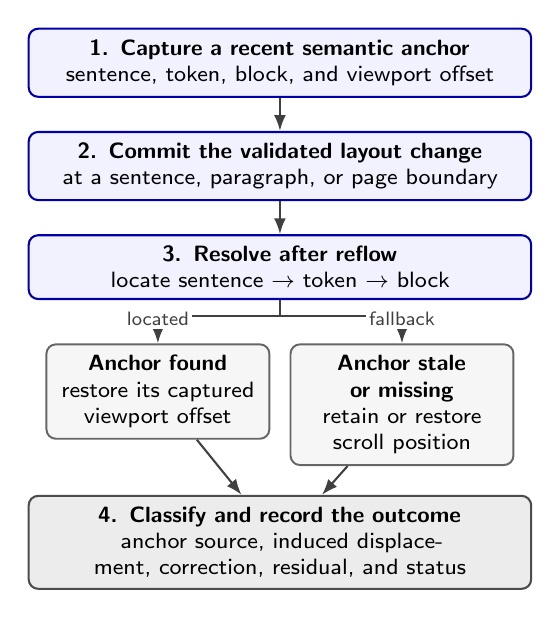
\begin{tikzpicture}[
        font=\footnotesize\sffamily,
        ctxstep/.style={rounded corners=1.2mm, draw=blue!65!black, fill=blue!5, line width=0.75pt, text width=6.1cm, minimum height=0.72cm, align=center, inner sep=4pt},
        branch/.style={rounded corners=1.2mm, draw=black!60, fill=gray!7, line width=0.7pt, text width=2.55cm, minimum height=0.82cm, align=center, inner sep=4pt},
        record/.style={rounded corners=1.2mm, draw=black!70, fill=gray!15, line width=0.75pt, text width=6.1cm, minimum height=0.76cm, align=center, inner sep=4pt},
        arrow/.style={-{Latex[length=2mm]}, line width=0.75pt, draw=black!75},
        edge/.style={font=\scriptsize\sffamily, fill=white, inner sep=1pt, text=black!75}
    ]
        \node[ctxstep] (capture) {\textbf{1. Capture a recent semantic anchor}\\sentence, token, block, and viewport offset};
        \node[ctxstep, below=0.42cm of capture] (commit) {\textbf{2. Commit the validated layout change}\\at a sentence, paragraph, or page boundary};
        \node[ctxstep, below=0.42cm of commit] (resolve) {\textbf{3. Resolve after reflow}\\locate sentence $\rightarrow$ token $\rightarrow$ block};
        \node[branch, below=0.55cm of resolve, xshift=-1.55cm] (found) {\textbf{Anchor found}\\restore its captured viewport offset};
        \node[branch, below=0.55cm of resolve, xshift=1.55cm] (missing) {\textbf{Anchor stale or missing}\\retain or restore scroll position};
        \node[record, below=0.7cm of found, xshift=1.55cm] (outcome) {\textbf{4. Classify and record the outcome}\\anchor source, induced displacement, correction, residual, and status};

        \draw[arrow] (capture) -- (commit);
        \draw[arrow] (commit) -- (resolve);
        \draw[arrow] (resolve.south) -- ++(0,-0.2) -| node[edge, near end, above] {located} (found.north);
        \draw[arrow] (resolve.south) -- ++(0,-0.2) -| node[edge, near end, above] {fallback} (missing.north);
        \draw[arrow] (found) -- (outcome);
        \draw[arrow] (missing) -- (outcome);
    \end{tikzpicture}
    \caption{Context-preservation sequence. The runtime captures a recent semantic anchor, commits a validated change at a reading boundary, locates the anchor after reflow, compensates its viewport offset, classifies the residual, and appends the outcome to the session record.}
    \Description{A four-step flow. The runtime captures a semantic anchor, commits a layout change at a reading boundary, resolves the anchor after reflow or falls back to scroll position, and records the displacement, correction, residual, and status.}
    \label{fig:context-sequence}
\end{figure}

Figure~\ref{fig:context-sequence} shows that restoration is instrumented rather than assumed.
The browser reports the anchor source, the displacement induced by reflow, the correction applied, the residual error, and a graded outcome.
An optional highlight briefly identifies the restored sentence.
Because the highlight and positional restore are distinct mechanisms, they should be manipulated separately in a future efficacy study.

\subsection{Authoritative Record, Export, and Replay}

The backend appends raw gaze and enriched semantic observations to one session record.
The same record contains eye-movement events, proposals, intervention lifecycles, restoration outcomes, and role-specific latency samples.
Periodic persistence workers write recovery chunks so an interrupted session can be exported as incomplete rather than silently lost.
At export, the system produces a schema-versioned full record, a processed representation that joins gaze to the latest semantic focus, and a telemetry record with latency distributions.
The content presented to a reader is included with a hash, and replay reconstructs the session from the exported timeline.

This record is the basis for the analysis in Section~\ref{sec:evaluation}.
It also exposes failures that a success-only event log would hide: rejected and expired proposals remain visible, and a restoration attempt records a residual even when its graded status is degraded.

\section{Evaluation}
\label{sec:evaluation}

We evaluate the platform as a research artifact rather than test the efficacy of an adaptive reading treatment.
The evaluation asks four questions corresponding to the design goals:

\begin{description}
    \item[EQ1:] Are module boundaries enforced and usable by built-in and external implementations?
    \item[EQ2:] Does the single-host deployment sustain the tracker stream with measurable quality and low local transport delay?
    \item[EQ3:] Does the intervention instrumentation reveal whether semantic context is preserved across reflow?
    \item[EQ4:] Does the platform retain enough evidence to reconstruct the relationship among gaze, decisions, interventions, and outcomes?
\end{description}

\subsection{Evaluation Material and Procedure}

The evidence combines automated tests and static architecture inspection, eight recorded reading sessions on real hardware, one separate advisory-path validation run, and a deterministic browser harness for layout displacement.

Four participants each completed one session with place-keeping enabled and one without, for eight sessions in total.
All sessions used a Tobii IS4 Large Peripheral tracker at a nominal 90 Hz on a 2560 by 1440 display.
The participant and researcher browsers and backend ran on one host, so all network measurements represent local loopback.
The eight sessions used the external analysis path and manual interventions; the advisory decision path was measured in a separate run.

The behavioral comparison is a feasibility pilot.
Condition order was imbalanced, intervention timing and type were selected by the researcher, exposure differed between conditions, and the enabled condition combined positional restoration with highlighting.
These choices are suitable for exercising the platform but not for estimating a treatment effect.

\draftnote{Before external circulation, confirm and insert the approved recruitment, consent, ethics-review or exemption, compensation, and data-reuse wording. The repository must remain private until the participant-data issue described in Section~\ref{sec:ethics} is resolved.}

\subsection{Modularity and Functional Evidence}

The backend's dependency direction is checked by an executable architecture test: core domain and application projects cannot depend on infrastructure or the Web API.
An in-process module can be introduced through one registration point, and the generic provider protocol was exercised by a reference decision provider, a reference eye-movement analyzer, and an adapter to an external reading-analysis pipeline.
These integrations cover both analysis and decision module types.

At the time of this draft, the current backend suite passes 101 tests and the frontend production build and lint checks succeed.
The reference decision provider passes three Python tests.
Eight tests in the reference eye-movement analyzer still encode a superseded provider protocol and fail against the current generic envelopes; the implementation and tests must be reconciled before the artifact is released.
The frontend has no automated browser test suite, leaving the gaze-to-token and context-restoration paths dependent on manual walkthroughs and the deterministic harness.

These results support the existence and use of the module boundary, but not every resilience behavior described in early design documentation.
In particular, the implementation advertises heartbeat timeouts without a watchdog that expires stale providers, and a provider disconnect updates status but does not automatically switch an active external strategy to its built-in counterpart.
We therefore do not claim automatic fallback or liveness enforcement.

\subsection{Sensing Quality and Local Latency}

Across the eight sessions, the export contains 175,860 gaze samples, 9,311 fixation events, 3,225 saccade events, and 45 manually initiated interventions.
Table~\ref{tab:runtime-results} summarizes the primary runtime measurements.

\begin{table}[t]
    \caption{Runtime measurements in the single-host laboratory deployment. Percentiles are empirical over recorded samples.}
    \label{tab:runtime-results}
    \small
    \begin{tabular}{lrrr}
        \toprule
        Measure & $n$ & Center & Tail / range \\
        \midrule
        Sampling rate (session) & 8 & 89.9 Hz mean & 89.41--90.06 \\
        Valid gaze (session) & 8 & 95.6\% mean & 92.47--98.01\% \\
        Inter-sample interval & 175,852 & 11.103 ms & 11.104 ms \\
        Participant client RTT & 387 & 1 ms & 3 ms \\
        Researcher client RTT & 393 & 1 ms & 8.4 ms \\
        Decision path, separate run & 14,015 & 6 ms & 11 ms \\
        Provider RTT, separate run & 8 & 4.5 ms & 6.3 ms \\
        \bottomrule
    \end{tabular}
\end{table}

The achieved sampling rate ranged from 89.41 to 90.06 Hz, with mean 89.9 Hz and standard deviation 0.2 Hz.
The fraction of samples in which at least one eye was valid ranged from 92.47\% to 98.01\%, with mean 95.56\%.
Calibration accuracy ranged from 0.296 to 0.685 degrees and successive-sample precision from 0.083 to 0.330 degrees.
The inter-sample analysis excludes intervals of 30 ms or more; 57 intervals (0.032\%) fall outside that plotting range and should be reported rather than silently treated as absent.

\begin{figure*}[t]
    \centering
    \begin{minipage}[t]{0.49\textwidth}
        \centering
        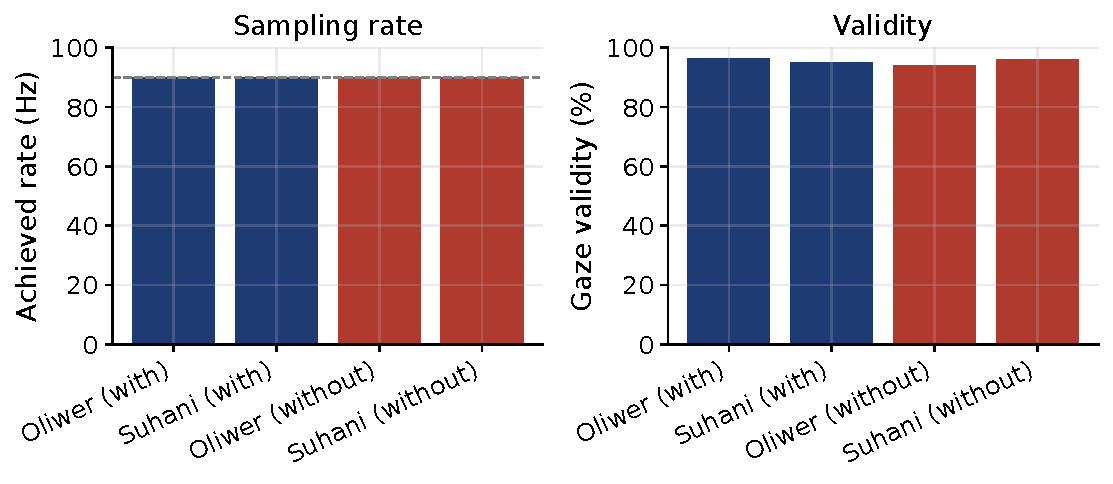
\includegraphics[width=\linewidth]{Chapters/07_Evaluation/eval-sensing-rate-validity.pdf}
    \end{minipage}\hfill
    \begin{minipage}[t]{0.49\textwidth}
        \centering
        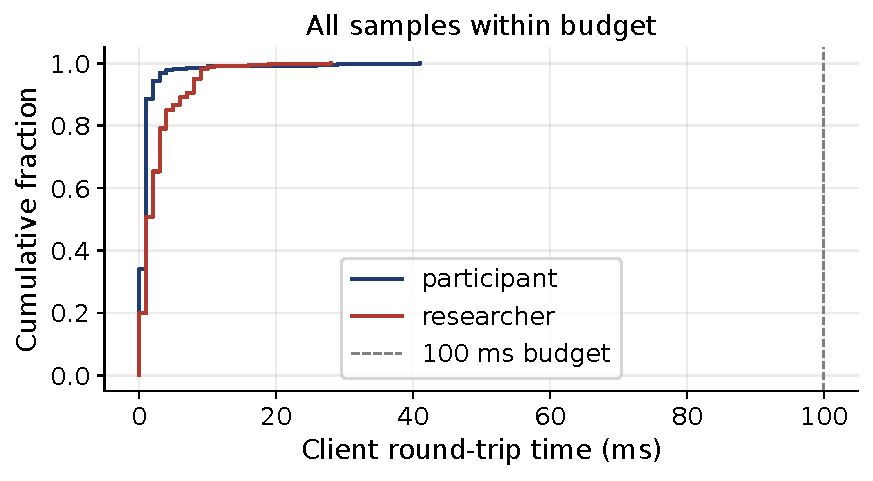
\includegraphics[width=\linewidth]{Chapters/07_Evaluation/eval-client-rtt.pdf}
    \end{minipage}
    \caption{Sensing and local transport measurements across the eight Tobii-backed sessions. Left: achieved sampling rate and gaze-validity rate. Right: participant and researcher client round trips on local loopback. These are transport measurements, not a gaze-to-visible-intervention latency.}
    \Description{Two charts. The first shows approximately 90 hertz sampling and 92.5 to 98 percent valid gaze across eight sessions. The second shows low local participant and researcher client round-trip times with all main-session values under 100 milliseconds.}
    \label{fig:runtime}
\end{figure*}

The main-session client round trips in Figure~\ref{fig:runtime} remained under the project's 100 ms transport budget.
This does not measure the full path from a gaze sample through analysis, decision, browser layout, and repaint.
The separate 91-second advisory run provides a narrower decision-path check: 14,015 recorded in-process evaluations had median 6 ms, p95 11 ms, and maximum 46 ms; eight external-provider round trips had median 4.5 ms and maximum 7 ms.
The reference provider ran on the same host and the measurement excluded browser repaint.
The count of decision-path observations exceeds the run's 8,004 gaze samples, so the instrumentation semantics and triggering frequency must be documented before this metric is treated as a per-sample latency.

\subsection{Restoration as a Failure-Detection Case Study}

Restoration telemetry was generated for 19 live place-keeping interventions.
Only three were graded preserved and 16 degraded.
Among degraded events, the median reported anchor residual was 389 px even though the median intervention-induced viewport correction was approximately 39 px.
The instrumentation therefore contradicted the intended behavior: the original semantic-restart strategy often moved the recovered sentence farther than the reflow itself.

Inspection identified the cause.
The original strategy aligned the recovered sentence to a fixed location near the top of the reading area.
For a small reflow this correction could be much larger than the displacement it was meant to undo.
The revised strategy instead retains the anchor's pre-change viewport offset.

The deterministic harness applies 11 layout interventions at six reading positions.
Committed summaries report median displacement of 34.3 px without restoration, 104.4 px with the original strategy, and 32.4 px with the revised strategy.
For visible complete pairs, 45 of 62 original cases and four of 63 revised cases lie above the equality line in Figure~\ref{fig:restore}.
However, the two restore versions were captured in separate browser runs and anchor identities differ in some cases.
The current aggregate is therefore diagnostic evidence, not a fully matched experiment.

\begin{figure}[t]
    \centering
    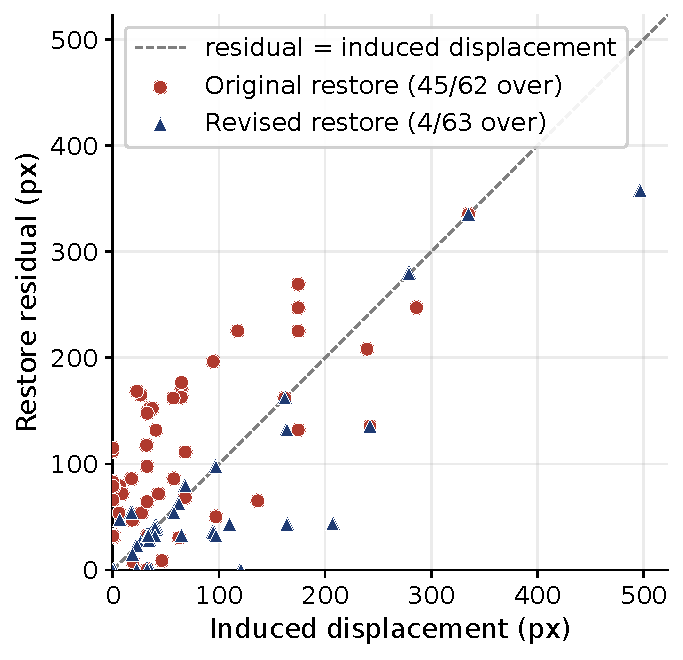
\includegraphics[width=0.94\columnwidth]{Chapters/07_Evaluation/eval-restore-overreposition-fixed.pdf}
    \caption{Deterministic displacement diagnostic for the original and revised restoration strategies. Points above the equality line indicate that restoration moved the anchor farther than the layout change alone. Counts use complete visible pairs (62 original; 63 revised). Because versions were captured in separate runs, the figure motivates rather than replaces a locked, matched rerun.}
    \Description{A scatter plot of induced displacement against residual displacement. Most original-strategy circles lie above the line of equality, while most revised-strategy triangles lie on or below it.}
    \label{fig:restore}
\end{figure}

\draftnote{Before submission, rerun baseline, original, and revised strategies in one pinned browser environment with commit, font, viewport, content hash, and stable anchor identity recorded for every trial. Replace Figure~\ref{fig:restore} and its statistics from that matched run.}

\subsection{Exploratory Reading Observations}

The feasibility sessions contained 19 interventions in the enabled condition and 26 in the disabled condition.
All 19 enabled interventions and 25 of 26 disabled interventions had a valid time to the next detected forward saccade.
The observed median time was 482 ms with place-keeping and 650 ms without it; means were 670 and 923 ms.
Mean per-intervention post-regression proportions were 22.8\% and 33.0\%, compared with pre-intervention values of 29.3\% and 32.0\%.
The per-participant median of this operational measure favored the enabled condition for three of four participants.

These values are exploratory for five reasons.
First, interventions are nested within only four participants.
Second, condition order was not balanced.
Third, researchers manually selected intervention timing and the number and types of interventions differ between conditions.
Fourth, the enabled condition combines a positional restore and a temporary highlight, so their contributions cannot be separated.
Fifth, time to the next detected forward saccade and regression proportion are operational proxies rather than measures of comprehension, reading recovery, or accessibility benefit.
We therefore report no hypothesis test or causal effect and do not use these observations as a paper contribution.

\subsection{Record Completeness and Analysis Readiness}

The raw session records and committed analysis cache agree on the principal eight-session counts and the descriptive forward-saccade timing summaries.
The processed exports demonstrate that gaze, semantic focus, proposals, interventions, context outcomes, and telemetry can be reconstructed from the authoritative record.
This supports EQ4 at the level of record content.

The current repository does not yet support a clean fresh-clone reproduction claim.
A root-level telemetry file is discovered as a full session by the analysis loader and causes a schema error; the analysis README also describes an earlier two-participant dataset, and committed cache files lack input hashes and freshness validation.
The paper artifact must therefore pin the Python environment, use an explicit session manifest, record source hashes, define event deduplication and missing-data rules, and regenerate every table and figure from raw de-identified inputs in one command.

\section{Discussion}

\subsection{The Contribution Is an Experimental Boundary}

The principal result is not that a particular intervention helps readers.
It is that the experiment runtime exposes the boundaries at which such a claim could later be tested.
Sensing quality is recorded before interpretation; analysis is replaceable; a decision remains distinct from its approval; an approved action remains distinct from its visible commit; and restoration reports a measured residual rather than a Boolean success chosen by the implementation.
This structure makes disagreements inspectable.

The restoration case illustrates the value of that boundary.
The initial mechanism appeared semantically reasonable because it found the same sentence after reflow.
Only the recorded pixel residual revealed that it often displaced the sentence more than the layout change did.
The resulting lesson generalizes beyond reading: an adaptive interface should measure the cost of realizing an adaptation, not only the quality of the model that requested it.

\subsection{Human Authority Is Part of the Architecture}

Manual, advisory, and autonomous modes share the same proposal and intervention records.
This lets a study move gradually from researcher control to automation without changing the presentation runtime or losing provenance.
Advisory mode is particularly useful while a decision provider is experimental: the researcher can approve or reject its output, and later analysis can distinguish model behavior from operator resolution.

The current implementation should not yet be described as resilient automation.
Provider identity validation is inconsistent across analysis and decision paths, heartbeat expiry is not enforced, and provider disconnect does not trigger automatic fallback.
These are artifact-hardening tasks and boundaries on the present claim.
The paper demonstrates modular connection and status visibility, not production fault tolerance or a secure multi-user service.

\subsection{Implications for Future Reading Studies}

The platform supports two complementary next studies.
First, the restore algorithm can be evaluated as a controlled systems component using a locked browser benchmark that treats the same anchors under baseline, original, and revised strategies.
Second, behavioral efficacy can be tested through a randomized, counterbalanced factorial design that independently manipulates positional restore and highlight.
Standardized intervention parameters and timing, multiple texts, comprehension outcomes, and participant-level modeling would be required before claiming that either mechanism improves reading.

The modular analysis port also permits comparison of the present geometric gaze-to-token heuristic with uncertainty-aware line assignment or other event detectors.
Such comparisons should report both assignment accuracy and the end-to-end consequences of uncertainty: delayed proposals, missed boundaries, and unnecessary interventions.

\section{Limitations}

The evaluation used one tracker model, one display configuration, and one single-host deployment.
Local transport measurements do not establish behavior over a network or under slow-client load, and the hot path has no explicit backpressure or sample-drop policy.
The platform manages one active experiment and is not a production multi-user service.

The browser's semantic mapping and the built-in event and decision strategies are heuristic.
They demonstrate the contracts but are not validated cognitive-state models.
No learned decision model was implemented, so support for AI-driven adaptation is architectural rather than empirical.
The collaborator integration shows that an external algorithm can cross the analysis seam, but model artifacts are not currently included and the adapter was written by the platform authors.

The behavioral pilot has only four convenience participants and the confounds described above.
The original restoration failed on small reflows; the revised strategy has preliminary geometric evidence but has not been tested with readers.
Frontend interaction paths lack automated browser tests.
Finally, the analysis and public-artifact pipeline require the reproducibility and privacy repairs described in Sections~\ref{sec:evaluation} and~\ref{sec:ethics}.

\section{Privacy, Ethics, and Artifact Status}
\label{sec:ethics}

Gaze traces can reveal reading behavior and may become identifying when combined with participant or device metadata.
The feasibility exports in the current private repository include direct identifiers and personal metadata that are not needed for the paper's analysis.
They will not be released in that form.
Before any public artifact, the authors will confirm the consent basis, ethics-review or exemption status, and permission for secondary publication use; remove or pseudonymize unnecessary fields; replace filenames with study identifiers; and assess removal from repository history.
A public package should contain only approved de-identified records, reduced aggregates, or a synthetic demonstration dataset, together with a clear data dictionary and retention statement.

\draftnote{This paragraph is intentionally conservative. Replace it with the institutionally approved 2--3 sentence privacy and ethics statement after review by the supervisors and the relevant DTU data-protection or ethics contact.}

\section{Conclusion}

Reading the Reader turns a sequence of gaze-contingent reading prototypes into an auditable experiment platform.
It separates sensing, analysis, decision, and intervention; gives a researcher live authority over proposals; stages validated typographic changes at reading boundaries; and records semantic restoration and latency alongside the gaze and decision evidence that produced them.
Eight Tobii-backed sessions show stable 90 Hz-class acquisition and low local transport delay in the intended laboratory deployment, while a restoration case study demonstrates how outcome instrumentation can expose a plausible but incorrect adaptation mechanism.

The present evidence supports the platform as a research instrument, not an efficacy or AI claim.
After the analysis pipeline, privacy controls, provider tests, and matched restoration benchmark are repaired, the artifact can provide a reproducible basis for controlled comparisons of gaze analysis, decision providers, and context-preserving typographic interventions.

\begin{acks}
Removed for anonymous review.
\end{acks}

\balance
\bibliographystyle{ACM-Reference-Format}
\bibliography{../Master-Thesis-Report/bibliography,references}

\end{document}
